% This file was created with tikzplotlib v0.10.1.
\begin{tikzpicture}

\definecolor{crimson2143940}{RGB}{214,39,40}
\definecolor{darkorange25512714}{RGB}{255,127,14}
\definecolor{darkslategray38}{RGB}{38,38,38}
\definecolor{forestgreen4416044}{RGB}{44,160,44}
\definecolor{lightgray204}{RGB}{204,204,204}
\definecolor{mediumpurple148103189}{RGB}{148,103,189}
\definecolor{sienna1408675}{RGB}{140,86,75}
\definecolor{steelblue31119180}{RGB}{31,119,180}

\begin{axis}[
axis line style={lightgray204},
height=0.45\textheight,
legend cell align={left},
legend style={fill opacity=0.8, draw opacity=1, text opacity=1, anchor=south east, draw=none},
tick align=outside,
tick pos=left,
title={Multi-Threaded Implementation Relative Execution Times},
width=\textwidth,
x grid style={lightgray204},
xlabel=\textcolor{darkslategray38}{Mesh size},
xmajorgrids,
xmin=-2150000, xmax=67150000,
xtick style={color=darkslategray38},
xtick={-10000000,0,10000000,20000000,30000000,40000000,50000000,60000000,70000000},
xticklabels={\ensuremath{-}1,0,1,2,3,4,5,6,7},
y grid style={lightgray204},
ylabel=\textcolor{darkslategray38}{Execution time relative to C++},
ymajorgrids,
ymin=0.584769215693879, ymax=1.71189604011066,
ytick style={color=darkslategray38}
]
\path [draw=black, semithick]
(axis cs:1000000,1)
--(axis cs:1000000,1);

\path [draw=black, semithick]
(axis cs:8000000,1)
--(axis cs:8000000,1);

\path [draw=black, semithick]
(axis cs:27000000,1)
--(axis cs:27000000,1);

\path [draw=black, semithick]
(axis cs:64000000,1)
--(axis cs:64000000,1);

\path [draw=black, semithick]
(axis cs:1000000,1.16155807824418)
--(axis cs:1000000,1.26821412480822);

\path [draw=black, semithick]
(axis cs:8000000,1.44300036800877)
--(axis cs:8000000,1.49130354896523);

\path [draw=black, semithick]
(axis cs:27000000,1.36986435112552)
--(axis cs:27000000,1.54511638145474);

\path [draw=black, semithick]
(axis cs:64000000,1.40538127443367)
--(axis cs:64000000,1.55097322881872);

\path [draw=black, semithick]
(axis cs:1000000,0.973622351332752)
--(axis cs:1000000,1.11847765284304);

\path [draw=black, semithick]
(axis cs:8000000,1.20765247313455)
--(axis cs:8000000,1.44228532116572);

\path [draw=black, semithick]
(axis cs:27000000,1.5145976824943)
--(axis cs:27000000,1.66066300263717);

\path [draw=black, semithick]
(axis cs:64000000,1.53130258066264)
--(axis cs:64000000,1.62224158840313);

\path [draw=black, semithick]
(axis cs:1000000,0.636002253167369)
--(axis cs:1000000,0.691474164472452);

\path [draw=black, semithick]
(axis cs:8000000,1.15526737082365)
--(axis cs:8000000,1.25933688492308);

\path [draw=black, semithick]
(axis cs:27000000,1.50103683366645)
--(axis cs:27000000,1.59975379366666);

\path [draw=black, semithick]
(axis cs:64000000,1.61589590433844)
--(axis cs:64000000,1.62677678024894);

\addplot [semithick, steelblue31119180, mark=x, mark size=3, mark options={solid}]
table {%
1000000 1
8000000 1
27000000 1
64000000 1
};
\addlegendentry{C++ with 1 OpenMP thread}
\addplot [semithick, darkorange25512714, mark=x, mark size=3, mark options={solid}]
table {%
1000000 1
8000000 1
27000000 1
64000000 1
};
\addlegendentry{C++ with 8 OpenMP threads}
\addplot [semithick, forestgreen4416044, mark=x, mark size=3, mark options={solid}]
table {%
1000000 1
8000000 1
27000000 1
64000000 1
};
\addlegendentry{C++ with 32 OpenMP threads}
\addplot [semithick, crimson2143940, mark=x, mark size=3, mark options={solid}]
table {%
1000000 1.21488606929779
8000000 1.46715199947357
27000000 1.45749032497406
64000000 1.47817730903625
};
\addlegendentry{Rust with 1 Rayon thread}
\addplot [semithick, mediumpurple148103189, mark=x, mark size=3, mark options={solid}]
table {%
1000000 1.04604995250702
8000000 1.32496893405914
27000000 1.58763039112091
64000000 1.57677209377289
};
\addlegendentry{Rust with 8 Rayon threads}
\addplot [semithick, sienna1408675, mark=x, mark size=3, mark options={solid}]
table {%
1000000 0.663738250732422
8000000 1.20730209350586
27000000 1.55039536952972
64000000 1.62133634090424
};
\addlegendentry{Rust with 32 Rayon threads}
\end{axis}

\end{tikzpicture}
